%%%%%%%%%%%%%%%%%%%%%%%%%%%%%%%%%%%%%%%%%%%%%%%%%%%%%%%%%%%%%%%%%%%
%                                                                 %
%                            CHAPTER ONE                          %
%                                                                 %
%%%%%%%%%%%%%%%%%%%%%%%%%%%%%%%%%%%%%%%%%%%%%%%%%%%%%%%%%%%%%%%%%%%

\chapter{INTRODUCTION} \label{sec:introduction}

Daylighting is the use of natural light and building geometry for aesthetically pleasing visuals and the creation of productive environments.
However, daylighting is more than just pleasing visuals and productive environments.
Daylighting is also an environmental sustainability design practice for creating greener buildings and reducing power consumption. %r1
Similarly, daylighting can also be seen as an  economic means to reduce a building's energy demands or increase worker productivity to generate capital. %r1
Despite the variety of definitions, daylighting will always refer to the use of daylight to meet an architectural purpose. %r1

% Overview 
Firstly, to understand what drives daylighting research a brief overview of daylight's advantages is necessary.
In short, daylight is mainly valued as a source of illumination; however, recent studies show that daylight also offers economic and health benefits.
%r1
Secondly, I explain why architects struggle with the design of daylighting systems.
By and large, daylighting is challenging by virtue of sunlight's dynamic nature.
Moreover, daylight used incorrectly can cause occupants both visual and thermal discomfort.
%
Lastly, I review architectural practices used in the design of daylighting systems for the purpose of better understanding current advances in daylighting research.
Briefly, architects exercise sketching techniques, follow rules-of-thumb, and consult daylighting visualizations to help guide the design of effective daylighting systems. 
%
All things considered, the motives that drive architects and building owners to employ daylighting systems also drive researchers to develop better tools for the design and analysis of daylight in architectural spaces.\\

% This section is basically done
\section{Benefits And Motivations Behind Daylighting Systems}
    
  % Our small intro into the next few pages of motives
  There are many benefits to using daylight over traditional electrical lighting.
  Recent studies show exposure to sunlight, offered readily through daylighting systems, has a variety of health benefits; benefits such as the stimulation of vitamin D production and maintenance of healthy circadian rhythms.
  In addition to health-related benefits there are economic motives that drive architects and building owners to implement daylighting systems.
  Some economic motives include increases in worker productivity and overall reducing energy demands.
  In short, daylighting system offer both economic incentives for building owners and health benefits for occupants.

  % TODO: Requires proof reading
  \subsection{Vitamin D}
    Vitamin D is an essential fat-soluble secosteroid required for healthy human functions. It aids in the absorption of calcium and other minerals. Vitamin D plays a significant role in the mineralization of bone\cite{Ross}.   
    Prolonged vitamin D deficiency can result in many serious diseases.
    Adults suffering from vitamin D deficiency can develop osteomalacia -- the softening of bones. Similarly, children deprived of vitamin D can develop harmful diseases such as rickets. Children diagnosed with Rickets suffer from poor bone mineralization and are prone to bone fractures and deformity\cite{Pettifor}. \\

    There are many way to meet daily vitamin D requirements. For example, skin tissue is capable of creating vitamin D on its own, certain foods contain high concentrations of the vitamin, and dietary supplements fortified with vitamin D are readily available\cite{Ross}.
    Human skin has a built-in mechanism that helps synthesis vitamin D through the exposure of Ultra Violet(UV) light. Light rich in UV hitting the surface of the skin will begin the processes of vitamin D synthesis. Synthesis through exposure to sunlight meets most people's daily vitamin D requirements. Foods we consume are usually rich in vitamin and minerals. However, vitamin D occurs in significant concentrations in very few natural food items, such as fatty fish, particular species of mushrooms, and beef liver.  Because of vitamin D's scarcity in naturally occurring food items and the harmful effects of deficiency vitamin D  in children, companies fortify common breakfast foods with vitamin D -- such as orange juice, milk, and cereals. Lastly, Vitamin D can also be taken in pill form as a deity supplement. \\

    Working typical office hours in windowless environments decreases exposure to daylight and increases the risk of vitamin D deficiency. Living an indoors lifestyle coupled with the widespread usage of sunscreen products, has created a vitamin D deficiency pandemic.  Our skin does not synthesize vitamin D efficiently. Wearing sunscreen with an SPF of 15 absorbs 99\% of UVB radiation and consequently, reduces the ability to synthesize vitamin D by as much as 99\%\cite{Holick}.
    Additionally, sunlight received through a glass window be non-helpful for vitamin D synthesis. Glass, while not a suitable form of total UV protection, filters out a percentage of UVB light\cite{tuchinda2006photoprotection} necessary for vitamin D synthesis. \\

    Architectural daylighting can help alleviate this risk by creating buildings with apertures\footnote{Apertures is an architecture term used to refer to opening in building, such as windows and skylights.} and geometries that promote deep penetration of natural lighting into a building's interior. Daylight is rich in UV radiation required for vitamin D synthesis.  Daylighting systems could, in theory, help keep occupants healthy by passively enabling occupants to meet their daily vitamin D requirements. \\

  % TODO: Requires proof reading
  \subsection{Circadian Photobiology}
    Daylighting has influence over our circadian photobiology. Circadian photobiology is the human experience of hormonal and behavioral changes throughout a roughly 24-hour cycle. The hypothalamic suprachiasmatic nucleus (SCN)  in the brain, which relies on input from non-rod/non-cone photoreceptor located in our retina, regulates these non-image forming light responses. These non-rod/non-cone photoreceptors are excited by the exposure to alternating periods of light and dark. They specifically respond to lighting conditions found in daylight\cite{Rea,Thapan}.\\

    Electrical lighting varies from natural daylight in a couple of biologically significant ways\cite{Rea}. Daylight offers a higher level of illumination, a wider spectrum of electromagnetic radiation, and a temporal variation in lighting. Firstly, sunlight in conjunction with skylight\footnote{Skylight is the diffuse illumination provided by sunlight scatted in the atmosphere.}, measures anywhere between 10 to 100 thousand lux\cite{Robbins}.
    However, the government agency of Occupational Safety and Health Administration (OSHA) set 322 lux as the minimum lighting requirement for typical office work\cite{OSHA}. Lighting conditions that do not excite photoreceptors responsible for maintaining our circadian rhythm, such as lighting conditions below 100 lux, are considered biological darkness\cite{Leslie,Rea}.
    % Barb r1  what is N? See Rea Paper Figure 5
    Secondly, the spectrum of light emitted by artificial lighting lacks the short wavelength electromagnetic radiation found in sunlight. Specific wavelengths of electromagnetic radiation significantly affects melatonin levels in humans. Melatonin suppression is important because it has significant influence in sleep-wake cycles, body temperature regulation, alertness, and blood pressure\cite{Gooley}. Studies show melatonin suppression varies most through the exposure to short wave electromagnetic radiation\cite{Brainard}. Consequently, daylighting systems offer the advantage of exposure to short wavelength electromagnetic radiation needed for melatonin suppression. Lastly, exposure to light during periods of the day asynchronous to our circadian rhythm can result in shifts in our sleep-wake cycles. These shifts, known as phase shifts, triggers melatonin suppression at specific times in our sleep-wake cycle. For instance,  morning light exposure triggers melatonin suppression resulting in the feeling of alertness\cite{Rea}. However, exposure to light at asynchronous times in our sleep-wake cycle results in a phase shift. An unexpected phase shift can have symptoms similar to jet lag and significantly hinder productivity\cite{Rea}. Daylight availability during those crucial morning hours could potentially have significant impact on employee productivity. \\

  % TODO: Requires proof reading
  \subsection{Increased Productivity}
    Studies show daylighting systems increase both the productivity and comfort of occupants\cite{Menzies}. Daylighting increases workplace productivity and satisfaction through a variety of means. To begin, the human eye as image processing system has evolved over millions of years to work optimally under full spectrum illumination provided by both sunlight and skylight. It is not surprising that the human visual system works better using daylight as a source of light compared to other sources of illumination. A visual task, such as reading, generally require less illumination from daylight than illumination from electrical lighting\cite{Robbins}. Additionally, daylight provides superior color rendering. Our visual system is tuned to differentiate colors under full spectrum illumination. Differentiating colors under low lighting conditions or fluorescent lighting is less accurate than differentiating colors under daylight\cite{Robbins}. There are current electrical lighting systems that provide full spectrum light, however, these systems are costly when compared to daylight. Moreover, occupants enjoy being near windows; Windows give occupants information about their outdoor environment -- including the time of day, weather conditions outdoors, and activities happening outside. Additionally, having a workstation near a window could evoke a feeling of importance in occupants. This feeling of importance increases worker satisfaction and could possibly increase productivity\cite{Leslie}. Overall, the satisfaction of occupants is important to architects and managers, because adverse environmental factors hinder productivity in a workspace.  \\

    %r1
    These productivity gains provide an indirect financial benefits to companies investing in daylighting systems. 
    Furthermore, focus groups and interviews with professionals involved in the architectural design process show that architects tend to prioritize the comfort, health, and productivity of occupants over a building’s sustainability\cite{Menzies}. However, careful design of daylighting systems can still provide large direct financial benefits by reducing power consumption.

  % TODO: Requires proof reading
  \subsection{Reduced Energy Demands}
    There are direct economic gains from daylighting systems. 
    Specifically, longterm energy conservation from reducing the usage of electrical illumination can save building owners significant capital.
    It is important to note that daylighting systems do not directly save capital, rather daylighting systems give building owners the opportunity to conserve energy by using sunlight as an alternative or supplement to electric illumination. In some cases, electricity companies charge peak hour rates during the afternoon when demand for electricity is at its highest. During these peak hours alternatives sources of light, such as daylighting, become cost effective.
    It is hard to estimate how much energy savings is possible by adding a specific daylighting system. Simulations are an important tool architects use to determine electrical demand during the design development processes.  Lighting usually accounts for about 25-40\% of a total building energy demands.
    According to one study daylight can save up to 52\% of energy on a wall adjacent to a window\cite{Leslie}.
    Adding windows to an architecture space doesn't always help reduce energy demand. Moreover, windows can even hurt energy savings via unwanted solar heat gain in the summer and heat loss in the winter. % more of this later
    \\

    Using daylight as an alternative or supplement to electrical lighting requires daylight management. Automatic daylight management consist of dimming systems that control the intensity of electrical lighting during peak hours when daylight is most readily available.  Some simulation results show that in the absence of daylight management power consumption from lighting can exceed 50\% of a building's total power demand.
    However, those simulations also show that daylight can reduce up to 18\% to 55\% of a building's heating and lighting demand\cite{Bodart}.
    Without a dimming system, the interval of time in which daylighting is cost effective is significantly reduced. Other simulation results showed energy savings of 60\% with daylighting coupled with automatic dimming control strategies\cite{Ihm}. 
    A major disadvantage of automated dimming systems is the lack of control of illumination and it's distribution. It is impossible to satisfy all occupants' personal illumination preference\cite{galasiu2006occupant}, as a result automatic dimming systems attempt to a meet generalized lighting requirement for a given space. This generalization might satisfy some occupants, but leave others uncomfortable.\\ 

    Also, dimming lights result in reduced thermal output from lighting fixtures\footnote{Thermal radiation produced from incandescent lighting generates significant amounts of heat, however, florescent and LED lighting are more efficient and do not produce comparable thermal output}. 
    Which in turn reduces the total cooling load required in space. The reduced cooling load also contributes to energy saving in daylighting systems\cite{Leslie}. 
    In addition to reducing the cooling load, daylighting can also be used for intentional solar heat gain during the winter, while preventing unintentional solar heat gain during the summer.
    Daylighting systems exploit the shallow sun angle in the winter season by using roof overhangs that let direct sunlight into a building during the winter months and blocking direct sunlight during the summer months. Heating a large space during the winter is expensive, and leveraging solar heat gain can aid in keeping heating cost down\cite{Bodart}. 
    Figure-\ref{fig:summer_winter}B illustrates how roof overhangs can be used to accomplish this common daylight energy saving technique.
    \\

% This requires some work r1
\section{Challenges Of Designing Daylighting Systems}
  
  % Unsure of apostrophe in "outnumbers design' affect"
  Daylight has many benefits over traditional electrical lighting, however,reaping those benefits is not effortless. There are many factors architects have to consider when designing a daylighting system. Choices made during the early design stage can have extensive impact on the effectiveness of a daylighting system. Likewise, design choices can also result in visual discomforts for occupants and economic loss for building owners. By and large, architects planning daylighting systems are required to analyze numerous designs' affect on daylight. Furthermore, architects have to be cautious of sunlight's dangers to both occupants and building owners.

  \subsection{Factors That Affect Daylighting}

    % [Introduction]
    Illumination of an architectural space via daylight is dependent on numerous factors including building-wide design choices, room-specific choices, and temporal variations.
    These factors make it difficult to assess the quality of a design in terms of daylighting.\\

    \paragraph{Building-wide Design Choices} 
    The cardinal orientation of a building is a choice that directly affects how daylight will illuminate architectural spaces. In the northern hemisphere, windows facing the south cardinal direction experience both direct sunlight and indirect skylight throughout the day. On the other hand, north facing windows do not experience only diffuse skylight. The opposite is true in the southern hemisphere. In the south, north facing windows experience both direct daylight and skylight and south facing windows experience only diffuse skylight. Likewise, windows facing east experience direct morning sunlight and windows facing west experience direct evening sunlight. The temporal variations in eastward and westward direct sunlight are due to the sun's westwards path across the sky\cite{Robbins}. See Figure-\ref{fig:north_south} for an illustration.

    \begin{figure}[h]
      \centering
      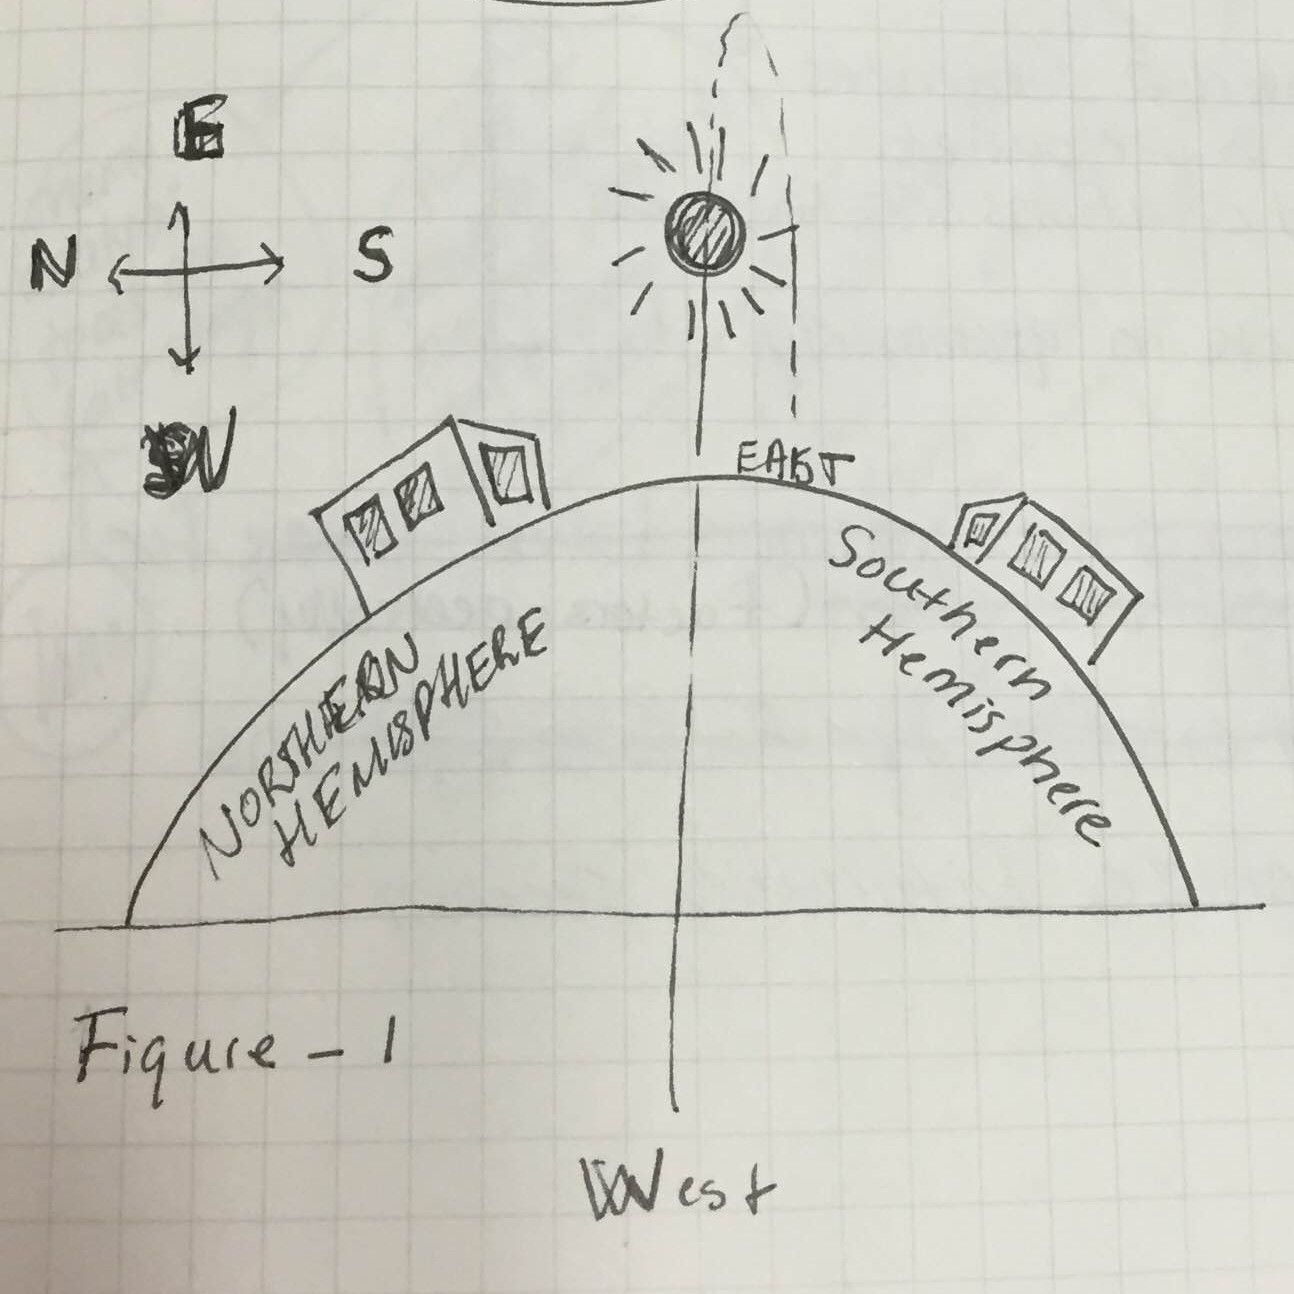
\includegraphics[width=0.25\textwidth]{north_south_fig}
      \caption{This illustration shows why windows facing southward in the northern hemisphere experience direct daylight and windows facing northward do not. It also shows the converse, north facing windows in the southern hemisphere experience direct lighting, however those facing southward do not.} 
      \label{fig:north_south}
    \end{figure}

    Aside from building orientation, building elevation can affect daylighting as well. Varying building elevation can change how daylight illuminates an architectural space. For example, a building located well above sea level will experience a slight difference in daylighting compared to a building below sea level. Daylight usually enters a space either perpendicular to a flat window pane or at a downwards angle starting from the Sun and ending at the floor and walls. However, a skyscraper could potentially have daylight enter a space at an upwards angle towards the ceiling due to its increased elevation.\\

    \begin{figure}[h]
      \centering
      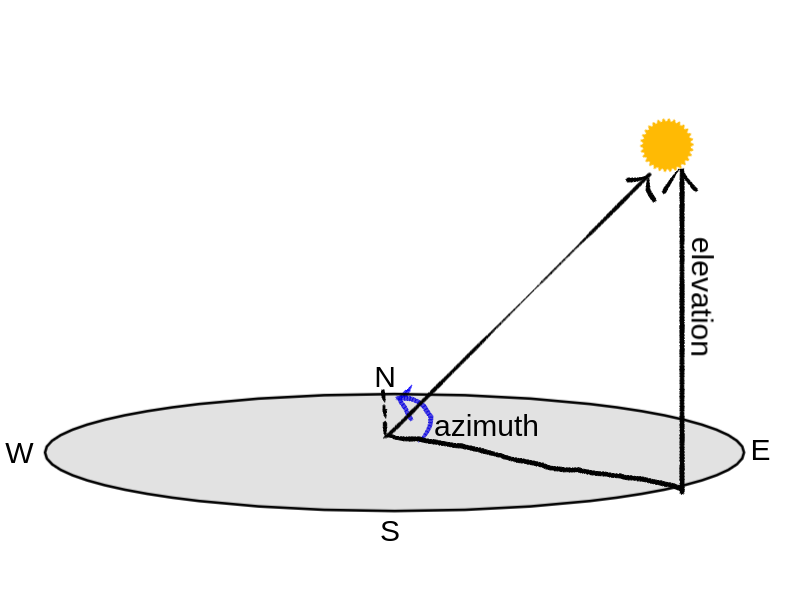
\includegraphics[width=0.5\textwidth]{sun_position}
      \caption{Illustration to show elevations and azimuth used to find the sun's position in the sky} 
      \label{fig:sun_position}
    \end{figure}

    \begin{equation} \label{eq:elevation}
    E = sin^{-1}(sin(\delta) sin(\phi) + cos(\delta) cos(\phi) cos(HRA))
    \end{equation}
    \begin{equation} \label{eq:azimuth}
    A = cos^{-1}( \frac{sin(\delta) cos(\phi) - cos(\delta) sin(\phi) cos(HRA)}{cos(E)})
    \end{equation}

    Equally important, the location of where a building is geographically built has direct impact on daylighting.
    Specifically, the path the sun travels across the sky varies with geographic location and time. 
    Equation-\ref{eq:elevation} and equation-\ref{eq:azimuth} are commonly used in daylighting to calculate the sun's position in the sky. 
    The elevation angle, given by Equation-\ref{eq:elevation}, is the angle between the horizon and solar zenith, as illustrated in Figure-\ref{fig:sun_position}. 
    $\delta$ in  equation-\ref{eq:elevation} and equation-\ref{eq:azimuth} refers to the solar declination angle. 
    Lastly, $\phi$ is the latitude of interest in both equations and $HRA$ is the hour angle in local solar time.
    The azimuth angle, as shown in Figure-\ref{fig:sun_position}, is the angle between the cardinal north direction and the direction projected sun from the horizon. The azimuth can be calculated once the elevation angle has been found, as show in equation-\ref{eq:azimuth}.
    As shown in both equations, the suns position in the sky is relative to longitude, latitude, and temporal variables.
    Similarly, surrounding vegetation and buildings can have influence of daylight in an architectural space. 
    For example, adjacent building can either occlude or reflect direct daylight into an architectural space, depending on the location and reflective proprieties of the nearby building. 
    Moreover, adjacent buildings not only occlude direct sunlight but also block access to skylight.
    The occlusion skylight can greatly reduce the amount of daylight available for use in architectural space.
    The same is true for vegetation. Trees, and similar vegetation, can be used to provide shade and diffuse harsh direct sunlight.
    \\

    % [Building design decisions]
    \paragraph{Room-specific Design Choices} 

    Room-specific design choices also have an impact on the daylight.
    The geometry of an interior space directly affects the distribution of daylight in a room.
    Geometries can be designed to diffuse direct lighting for uniform illumination and occupant comfort, as illustrated in Figure-\ref{geometry_sketch}.
    Similarly, shading devices and material properties of interior objects can affect daylighting.
    Shading devices, such as blinds can not only help diffuse direct lighting but also help redirect lighting up towards the ceiling, where it can be diffusely reflected back down towards occupants.
    Also, a careful selection of both the color and the material of interior items such furniture, walls, and ceiling can affect the distribution of daylight in an interior space. 

    \begin{figure}[h]
      \centering
      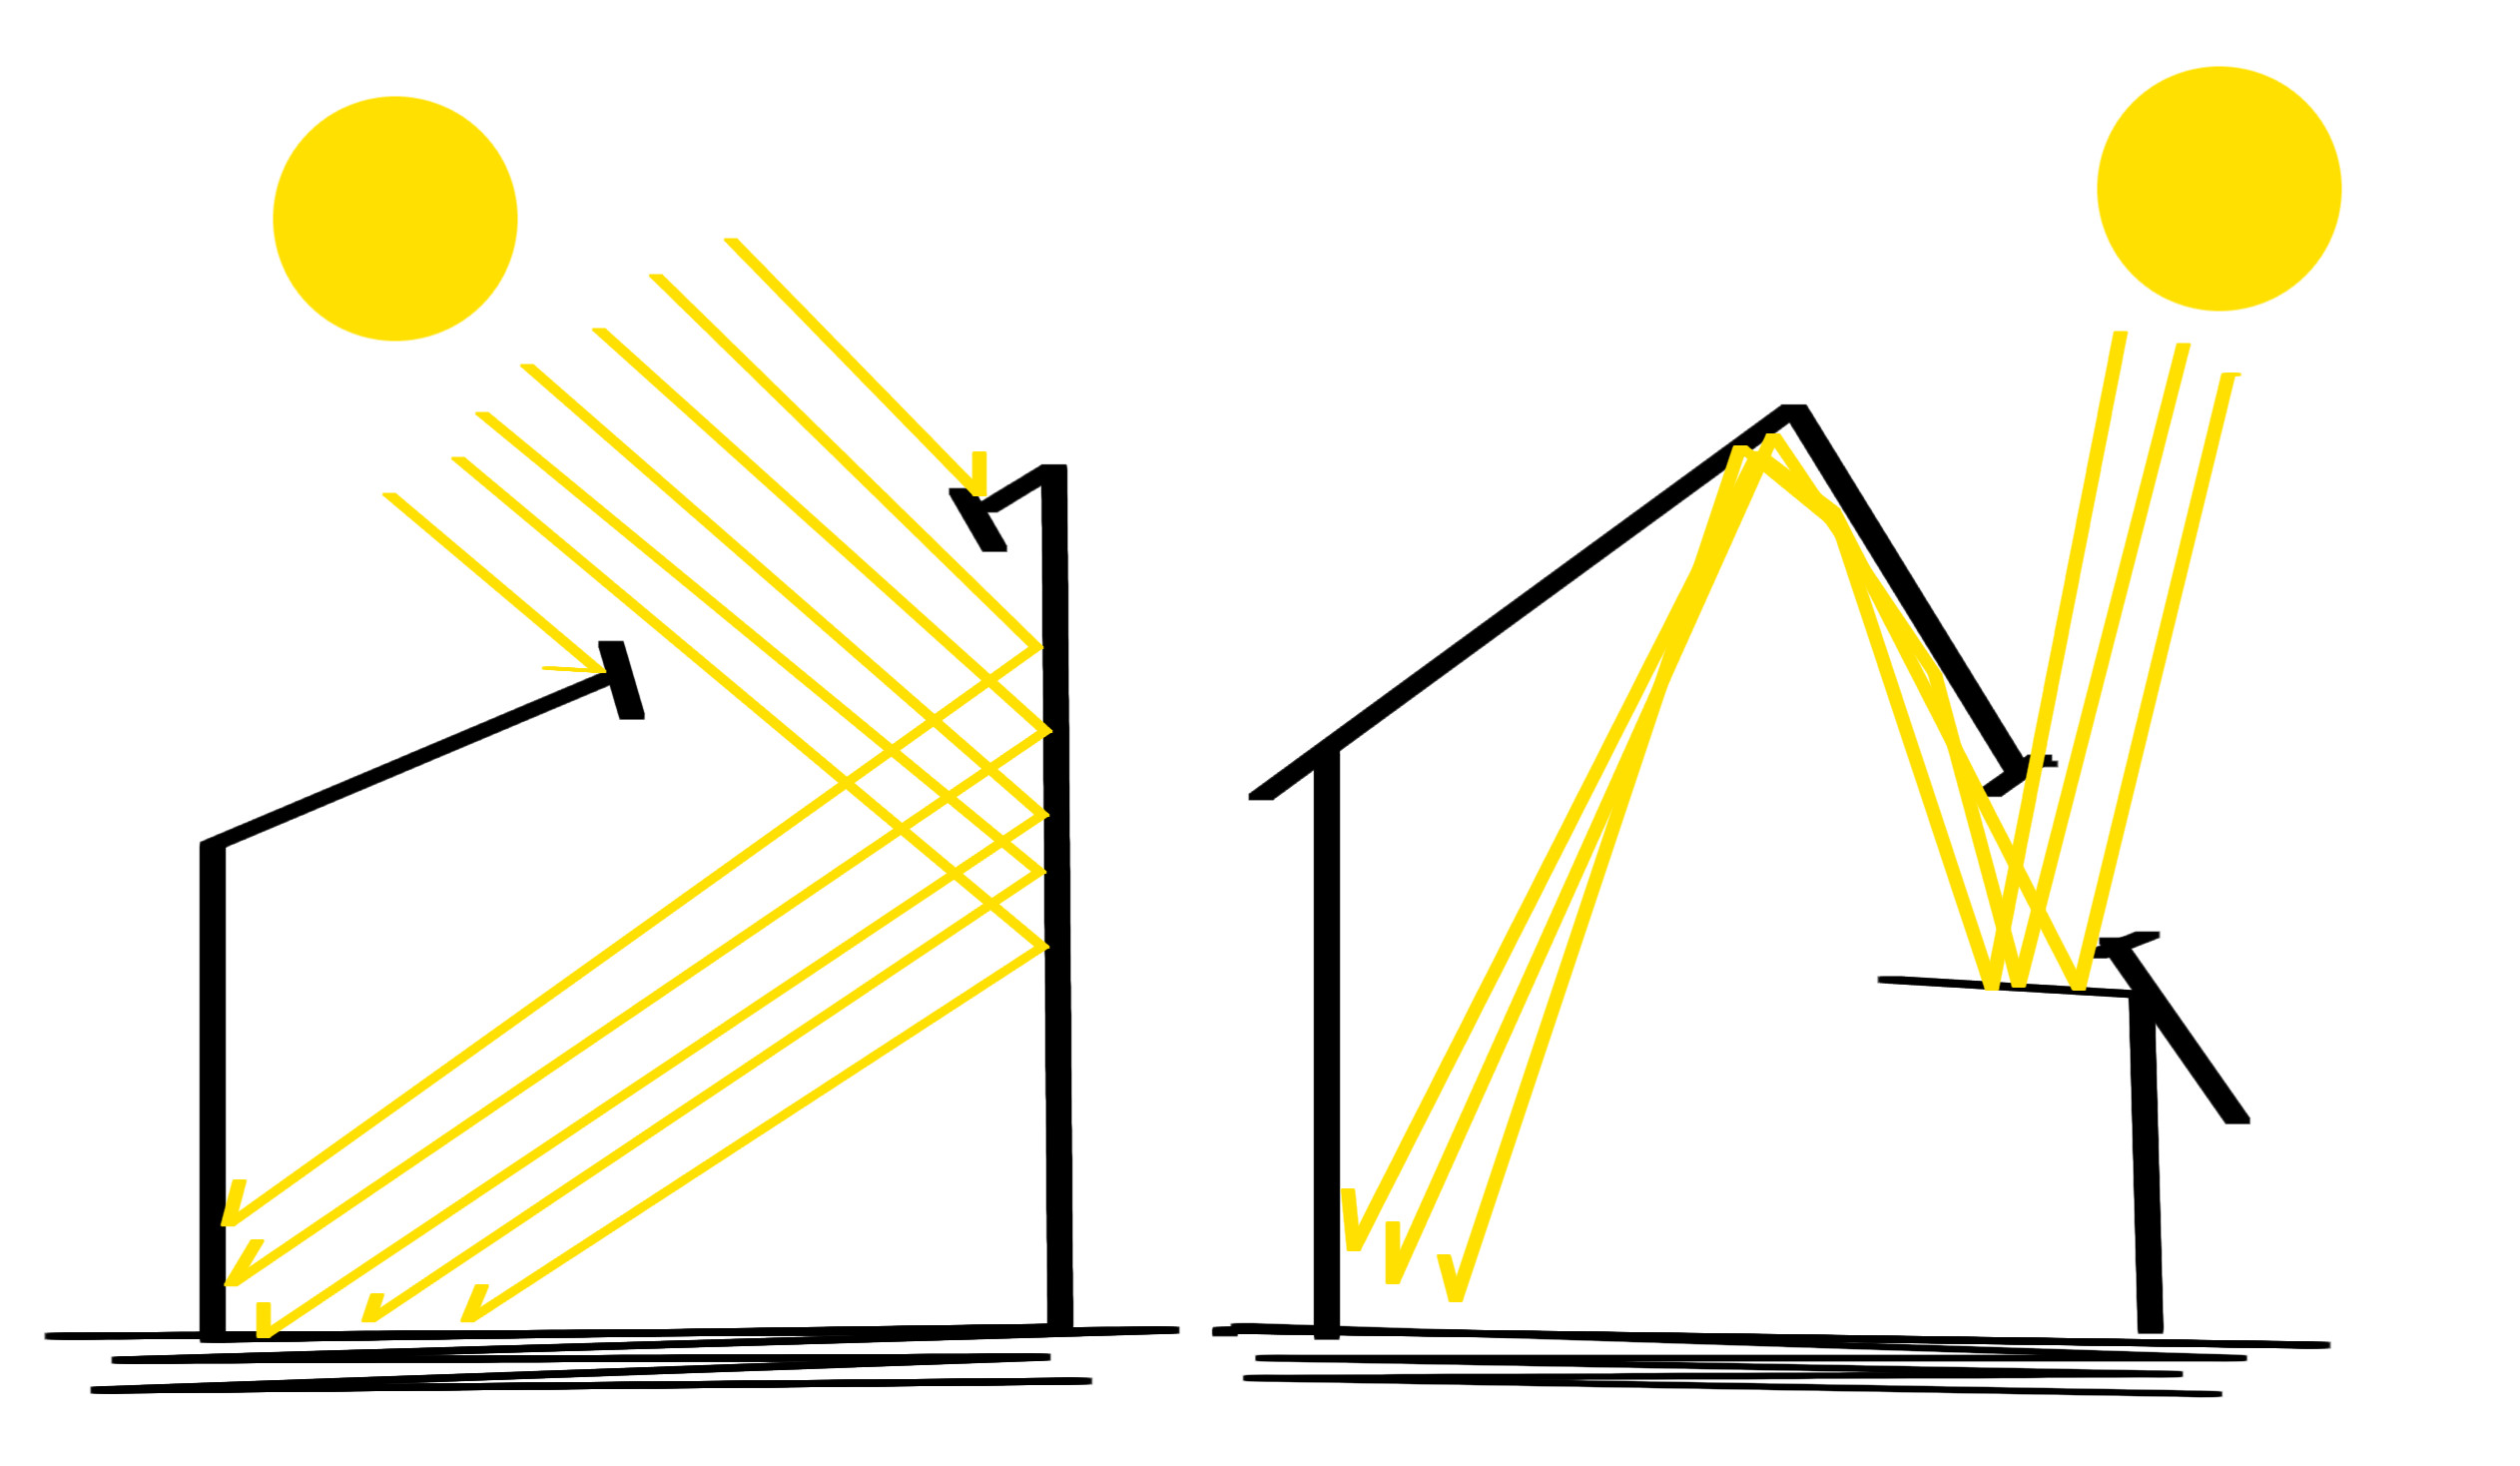
\includegraphics[width=0.5\textwidth]{geometry_sketch}
      \caption{Left: a common skylight placement on the roof of a building. The angled roof is designed to let daylight diffuse as it reflects on towards the floor. Right: A light shelf that helps redirect daylight up towards the ceiling, where it can be diffused and reflected back down on towards the floor.}
      \label{fig:geometry_sketch}
    \end{figure}

    In addition to material and shading devices, window placement and size directly influence daylighting.
    Larger windows and skylights allow more light to enter a space; however, these windows pose the risk of over-illumination and glare for occupants inside.
    Likewise, the glazing material used to treat windows can also be used to control the amount and distribution of daylight entering a space.
    The glass used in commercial buildings are glazed to block a significant portion of light from entering a space.
    Glazing are used because direct sunlight would cause over-illumination, thermal discomfort, and harm to the occupants situated near windows.
    Special glazing can also be used to help diffuse lighting up towards the ceiling and away from occupants.
    The choices that architects make in room-specific design significantly affect daylighting.\\

    % [Temporally]
    \paragraph{Temporal Variation} 

    It is obvious that daylight varies from sunrise to sunset.
    Less obviously, daylight also varies throughout the year.
    The sun's position in the sky is shallower during winter season than in the summer season. 
    Due to this, during the winter months daylight enters a room at a shallower angle, allowing light to travel deeper than in the summer months.
    Figure-\ref{fig:summer_winter}A illustrates the difference in light penetration during the winter and summer months.

    \begin{figure}[h]
    \centering
    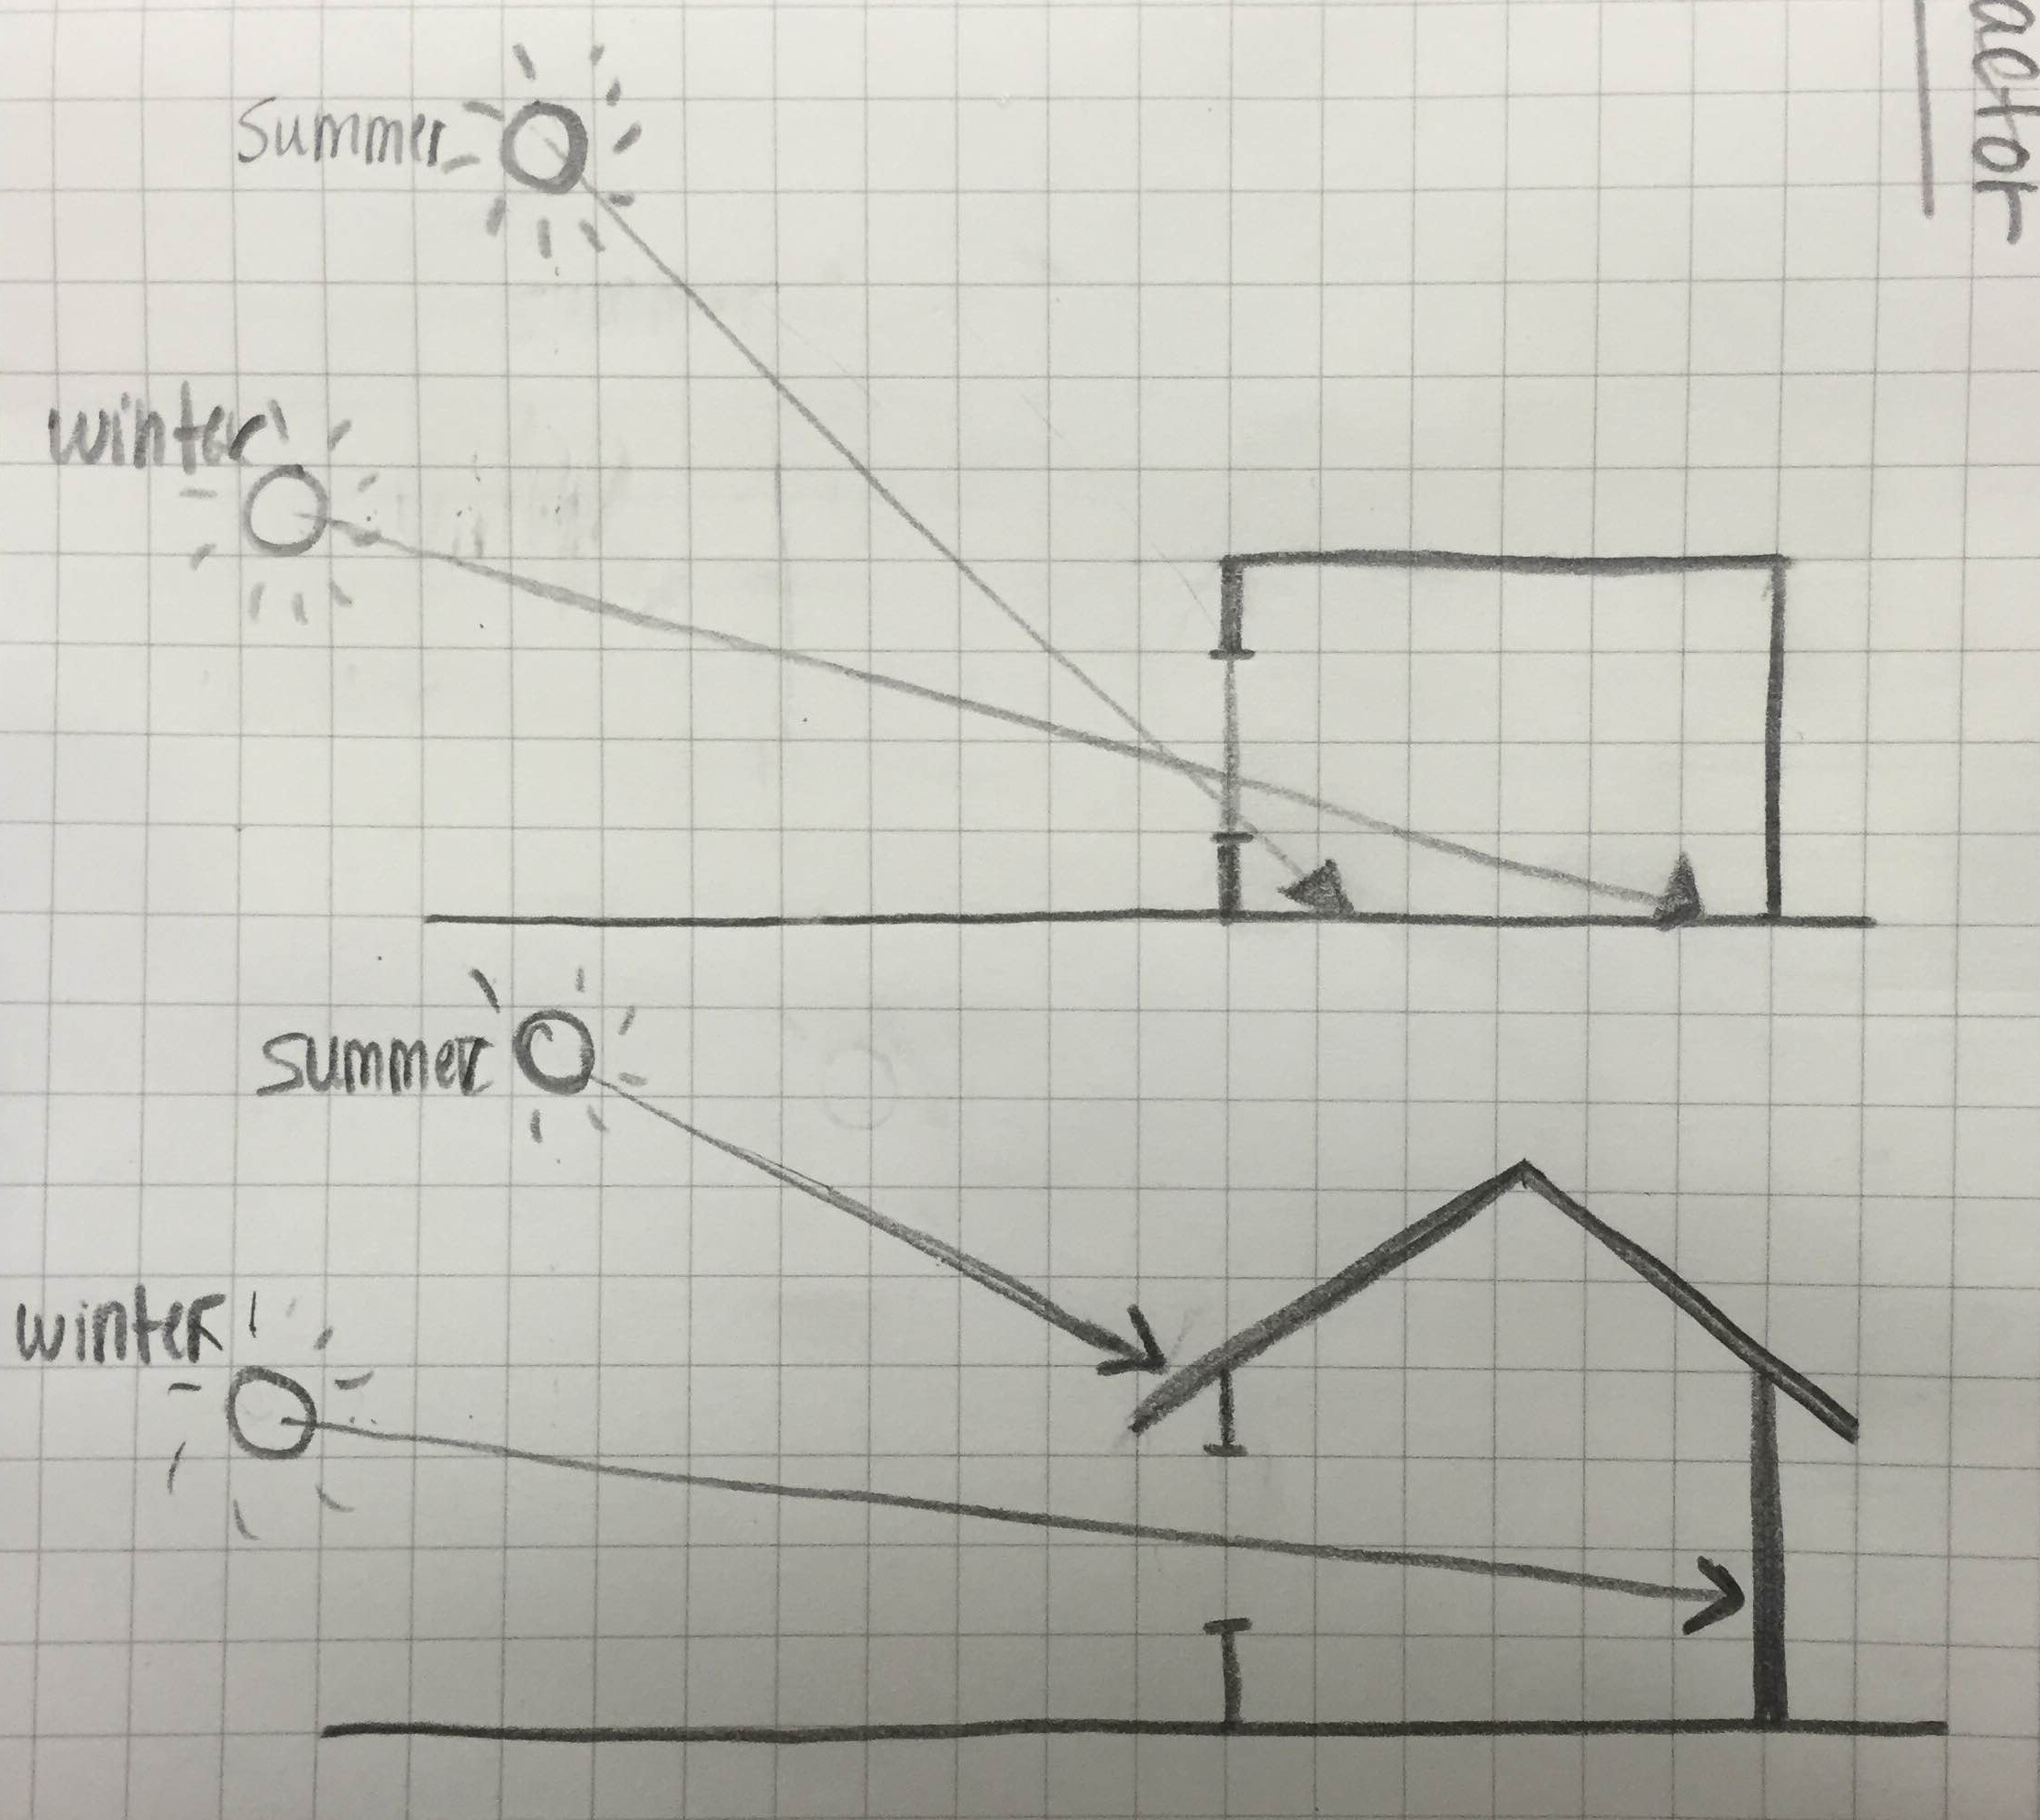
\includegraphics[width=0.5\textwidth]{summer_winter}
    \caption{Top: illustration to visualize the difference in light penetration during the winter and summer seasons. Bottom: a common daylighting technique is extending the roof to block light during the summer season, but not during the winter season.}
    \label{fig:summer_winter}
    \end{figure}

    As stated previously architects interested in sustainability, exploit this by extending the roof thus allowing daylight to enter during the winter and blocking direct daylight during the summer as shown in Figure-\ref{fig:summer_winter}B.
    Weather conditions also play an important role in the distribution and intensity of daylight. 
    During clear days, direct sunlight can enter a room and cause over illumination and glare.
    However during cloudy days, sunlight is diffused by clouds resulting in diffuse daylight.
    Weather conditions also vary by location, for example in upstate New York, cloudy skies are common, however in Florida clear skies are more frequent.
    % ASK_BARB: I think solar isolation means something else...
    A daylighting systems would be more efficient in locations with clearer skies then in locations where clear skies are uncommon.\\

    In brief, daylight varies depending on temporal factors, room-specific design choices, and building-wide decisions. These numerous factors make the distribution of daylight in a architectural space non-trivial to predict. 
    These difficulties pose a real challenge in the design of effective daylighting systems.

  \subsection{Adverse Daylighting Effects}

    As previously discussed, daylighting systems offer occupants a variety of benefits. However, poorly implemented daylighting systems can result in discomfort to occupants and increases in energy demand.

    \paragraph{Occupant Discomfort}

    % Over and under illumination
    Human vision can be understood and compared to an image processing systems.
    We require strong contrast and ample illumination to be able to clearly view and process symbols.
    The performance of visual task, such as reading, varies depending on the illumination and the clarity of the symbols being read.
    Under-illumination can make reading difficult and reduce worker productivity\cite{boyce}.
    Moreover, under illumination can occur in daylighting systems when daylight available is below a threshold to perform a specific visual task.
    The Occupational Safety and Health Administration (OSHA) set mandatory minimums on illuminations for common environments including offices, hallways, and warehouses to name a few;
    offices for example require a minimum of 322 lux.
    % Extension: Add in how we compute lux
    Similarly, hallways and warehouses have lower minimums set because there is no need to focus on fine details for prolonged periods of time\cite{OSHA}. \\

    Another visual discomfort that can occur from poor daylighting is glare.
    Glare is a reduction of contrast due a disproportionate amount of illumination from glare sources compared to illumination on a visual task.
    % Introduce the glare index
    Glare is hard to account for in the early design stages of architecture because glare is not only dependent on the source of illumination but also on viewpoint.
    Specifically, there are two main forms of glare -- disability glare and discomfort glare\cite{Robbins}.
    Disability glare occurs when a glare source is intense enough that it rendered the viewer momentary blind. 
    This kind of glare commonly occurs when driving at night and cars are passing in the opposite lane. 
    The strong light emitted from headlights would reduce the contrast of the road ahead and might result in momentary blindness.
    %
    Likewise, discomfort glare is similar to disability glare but much less dangerous. 
    Discomfort glare is also caused from bright glare sources, such as the sun or light reflected from the sun.
    Unlike disability glare, discomfort glare does not cause momentary blindness.  
    However prolonged exposure to discomfort glare when focusing on a visual task can significantly reduces both worker productivity and worker satisfaction\cite{boyce}. 
    Another visual discomfort, common in office environments, includes veiled reflection.
    Veiled reflections are the result of light reflecting off a surface directly into the eyes of the viewer. 
    For example reading an article from a glossy magazine in direct sunlight is challenging because at certain viewpoints the gloss on the page reflects light into your eyes reducing the contrast between both the black and white letters. 
    Veiled reflections, like glare, are difficult to predict because they are viewpoint dependent. \\

    Lastly, occupants sitting near windows can experience thermal discomfort at certain times of day.
    Daylight can be useful in warming up a space during the winter; however, daylight can also cause discomfort during the summer. \\

    Overall, there are various ways daylight can have adverse effects on occupant's comfort. As a result architects invest significant time and effort in daylighting analysis to prevent occupants from experiencing these adverse effects.
    Not only can occupants experience discomfort, but building owners can suffer economic loss from improperly created daylighting systems.

    \paragraph{Economic Loss}
    
    Another possible adverse product of daylighting systems is unintended solar heat gain. Solar heat gain is the increase in temperature inside a space due to daylight. 
    If too many windows are installed in particular location, a room can experience unintended solar gain.
    To counter solar heat gain, cooling systems must work at higher loads then usual resulting in increased energy usage.
    Furthermore, windows unless insulated well can result in heat loss during the winter seasons and nights.
    There several strategies architects can use to mitigate heat loss during the night.
    For example using thick drapes, shades, and shutters can provide layers of insulation to keep warm air inside from direct contact with the colder window.
    Additionally, there are specialized window glazing available the can help reduce heat loss during the winter and night.
    Ultimately, rooms with many windows might provide ample daylight during the daytime but carry the risk of significant heat loss during chilly nights and the winter months.
    \\

    Lastly, occupant behavior can result in the lost of investment capital for building owners.
    Occupants exposed to the visual discomforts of daylight can choose to use window blinds to block daylight out entirely and rely solely on electrical lighting.
    The use of electrical lighting, given available daylight, results in reduced energy savings for building owners.
    As mentioned previously, daylighting coupled with automated dimming systems can help prevent occupants from the visual discomforts of over illumination.
    However, having no control over automated dimming systems can cause occupants discomfort and result in coup d'\'{e}tat in which occupants only rely on electrical lighting.%there is no source, but it's too good to leave out.. 
    \\

    Moreover, daylighting systems are expensive to design and implement and as a result the initial cost is generally greater then using traditional electrical lighting.
    If occupants continuously choose electrical lighting over daylight, the break even point of the initial investment in a daylighting system is pushed back further -- essentially costing the building owner capital.
    Architects are then faced with the challenge of not only making visually pleasing lighting conditions, but also avoiding discomforts caused by daylight.

% This section needs to be written
\section{Daylighting In The Architectural Design Processes}

  % Explain that architecture of a building is big task that requires breaking down
  The architectural design of a building from concept to construction is no easy task.
  As a result, architecture firms and schools generally break down the architectural design process into five manageable phases\cite{bazjanac1974architectural}.
  % Explain how we will mainly focus on the early design stages
  Daylighting affects all phases of the architecture design process; however, choices made early in the design of an architectural space lays the foundations of a daylighting system.
  % Explain how daylight also has impact in how later phases are done,
  % - but that we do not focus on those stages
  Our focus lies in the early stages of the design processes: the schematic design phase.
  Nevertheless, we will briefly cover all of the architectural design process to give the reader a better understanding on the significance of the schematic design phase.

  \subsection{The Five Phases Of The Architectural Design Processes} 
  % List out the five stages
  The five phases of the architectural design process are: the schematic design phase, the design development phase, the construction documents phase, the bidding phase, and the construction administration phase.
  % NOTE: you do not have to give an explanation or connection to daylighting
  % Go over in (1) sentences the stage 1
  During the schematic design phase architects consult with clients to understand project specification and goals. Architects then produce drawings, sketches, and scale models of possible designs to show the client.
  % Go over in (1) sentences the stage 2
  A design from the schematic design phase is expanded upon in the design development phase.
  More details are added to the sketches, window placements are defined, and utility systems are laid out.
  % Go over in (1) sentences the stage 3
  With client approval, architects then begin creating formal construction documents. During the construction document phase, architects generate documents that are later used by contractors as blueprints.
  % Go over in (1) sentences the stage 4
  Once the blue prints are complete architects search for possible construction contractors.
  During the bidding phase architects take bids from contractors interested in the project.
  % Go over in (1) sentences the stage 5
  After contractors are found the architects oversee the construction project.
  This final phase of the architectural design processes is known as the construction administration phase.
  % Recap why I had to go over this
  Daylighting plays a role in each phase of the architectural design process, however, the choices made in the schematic design stage lay the foundation for an efficient daylighting system.

  \subsection{Daylighting In The Early Design Phase}
  % Explain that there are many techniques and tools architects use during this early design phase.
  During the schematic design phase architects employ a variety of strategies and techniques to guide their designs for the optimal use of daylight.
  % Brief overview of those including rules-of-thumb, sketch-analysis.
  Firstly, rules-of-thumb and simple calculations are used during the early stages of design, when building form, space, and order are conceptualized.
  Secondly, architects can analyze sketches to predict the distribution of daylight in interior spaces.
  % Small explanation as to why these tools are good (aka fast and easy)
  With enough practice sketching becomes a fast and easy way to express visual concepts.
  As a result, sketching is still the main medium during the early design phase, when being able to quickly express ideas is crucial.

  \paragraph{Rules-of-Thumb}

  \begin{figure}[h]
  \centering
  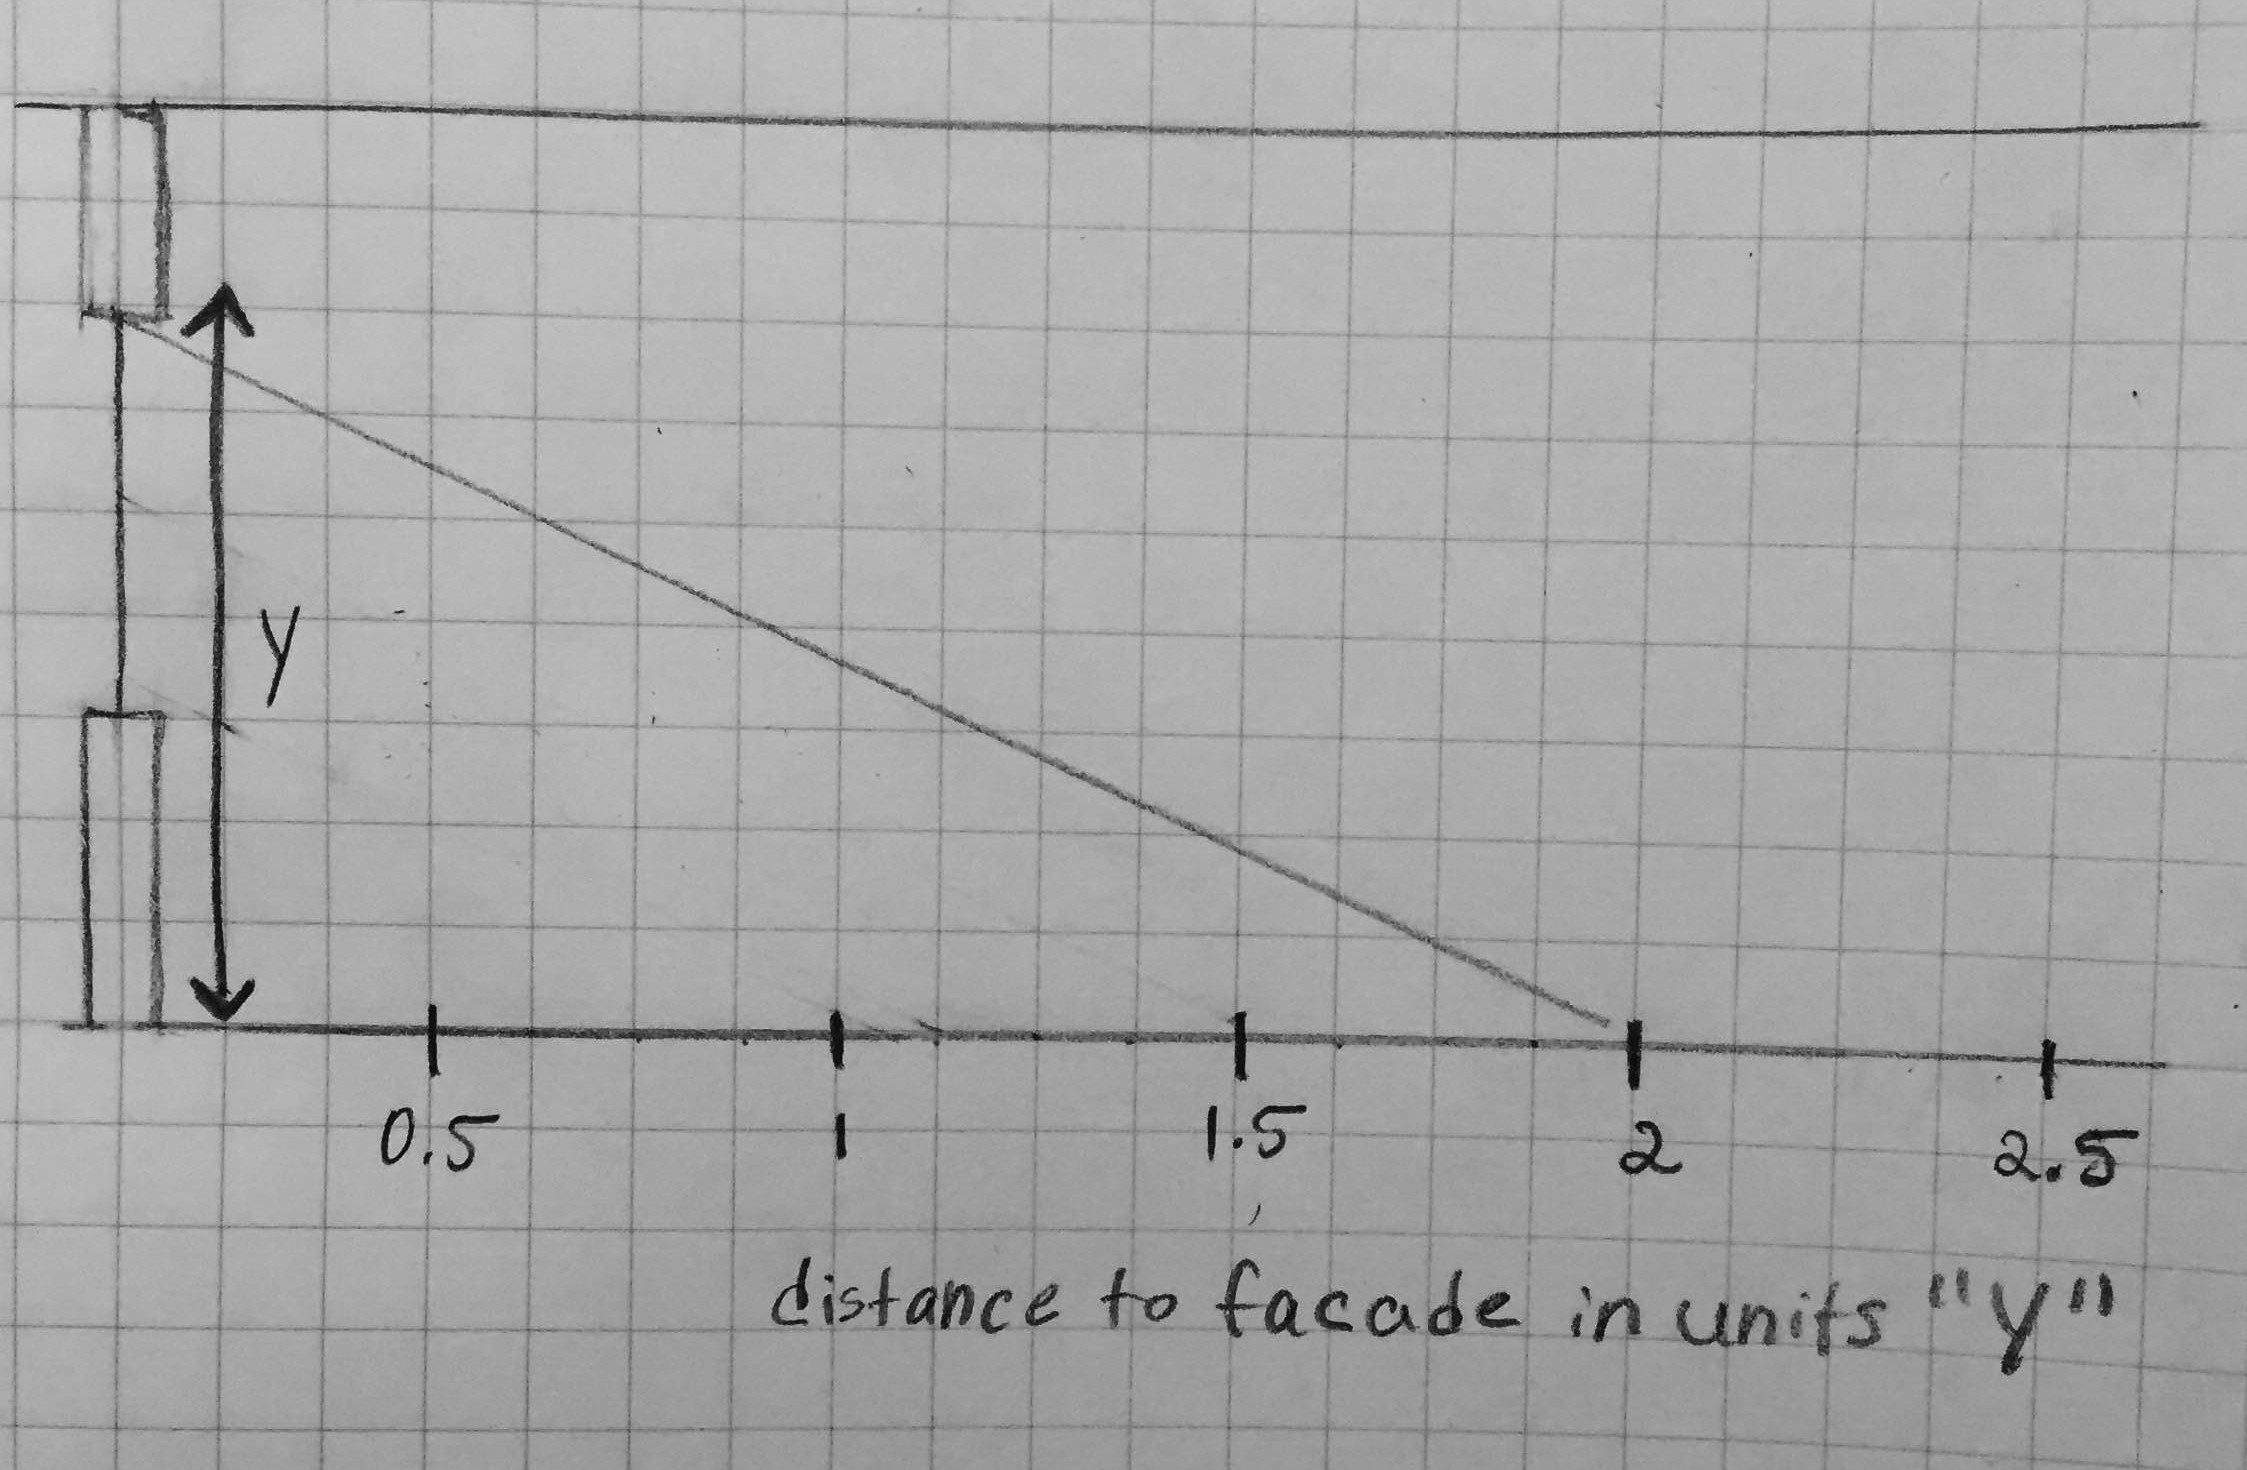
\includegraphics[width=0.5\textwidth]{rule_1}
  \caption{Verified rule-of-thumb: The depth of usable daylight is 1.5 to 2 times the window-head-height. Here the window-head-height is depicted as $y$.}
  \label{fig:daylightzone}
  \end{figure}

  % Explain what rules of thumb are
  A rule-of-thumb is a general suggestion, usually acquired through experience, that architects follow when designing spaces. 
  Many rules-of-thumb are widely accepted in practice, however, few have been validated\cite{reinhart2005simulation}.
  Furthermore, many designers using these rules-of-thumb do not have an understanding of the underlying principles behind them\cite{Galasiu}.
  Nevertheless, these rules are still used in practice because they are generally effective and straightforward to apply during the early stages of design.

  %%%% Rule 1
  Some common rules-of-thumb include simple suggestions about where to locate people within a space.
  For example, it is suggested that designers take advantage of the floor area within the daylight zone by situating people within it\cite{Leslie}.
  Moreover, architects suggest visual tasks be placed near the parameter of a building\cite{Leslie}.
  To elaborate, the daylight zone is a range of space where daylight can comfortably illuminates a workspace. 
  The daylight zone does not take direct daylight into consideration, but rather diffuse skylight.
  A validated rule-of-thumb is regularly used to find the rough range of the daylight zone\cite{reinhart2005simulation}. 
  The daylight zone extends to about 1.5 to 2 times the window-head-height\footnote{The window-head-height is a term that refers to the height from the floor to the top of a window.} away from the wall containing the window, as illustrated in Figure-\ref{fig:daylightzone}.

  %%%% Rule 2
  % Preferred facade for daylighting: south and north
  Another common rule-of-thumb is the elongation of the east-west axis of a building.
  The elongation of a building along the east-west axis is design choice meant to avoid solar heat gain and create more room for north facing windows\cite{Leslie}.
  As explained previously, north and south facing windows, depending on your location, can provide either day-round diffuse or direct daylight.
  However daylight from east and westward windows vary significantly throughout the day.
  Consequently, another general rule-of-thumb is that south and north facing windows are the preferred over east and westward windows\cite{reinhart_lecture}.

  %%%% Rule 3
  % Use light-colored interior surfaces. 
  % Light surfaces reduce the luminance contrast between the windows and surrounding surfaces, increasing visual comfort.
  Daylight distribution and comfort within an interior space depends on more than just window placement and size.
  A general rule-of-thumb is that light colored interior surfaces help reduce the contrast between windows and the interior of a space\cite{Leslie}.
  % desirable reflectance to have a well daylight environment:
  Moreover, the reflectance property of walls, windows, floors, and furniture impact daylight distribution.
  One more rule-of-thumb is that the ceiling should have a reflectance of at least 80\%, walls of at least 50-70\%, floors of at least 20-40\%, and furniture of at least 25-45\%\cite{reinhart_lecture}.
  % Summarize the rules of thumb and how many are guidelines.
  It is important to note that rules-of-thumb, while not all formally validated, help guide daylighting design.
  The straightforwardness of these suggestions and the ability to abstract away the complexities of daylight make rules-of-thumb an invaluable tool to building designers.

  \paragraph{Sketch Analysis}
  % Two example figures of daylighting used on sketches
  \begin{figure}[h]
    \centering
    \begin{minipage}[b]{0.4\textwidth}
      \centering
      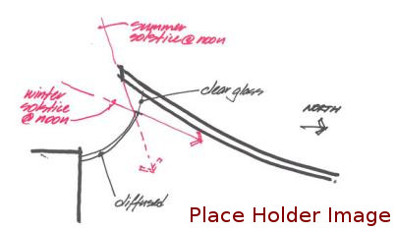
\includegraphics[height=0.5\textwidth]{yancy}
      \caption{Example of brainstorming daylighting on sketches}
      \label{fig:yancy}
    \end{minipage}
    \hfill
    \begin{minipage}[b]{0.4\textwidth}
      \centering
      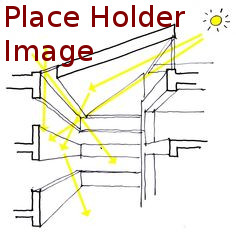
\includegraphics[height=0.5\textwidth]{digital_sketch}
      \caption{Example of brainstorming daylighting on sketches}
      \label{fig:digital_sketch}
    \end{minipage}
  \end{figure}

  % Explain that sketches are important in general in architecture
  Sketches are the primary medium architects use to convey visual ideas during the schematic design phase.
  % Explain that they are important in daylighting for general problem solving
  Sketches help externalize concepts and ideas for both problem solving and rough daylight analysis\cite{Suwa,yancy}.
  It is not surprising that sketches are also widely used in the brainstorming of daylighting system.
  % - reference the figures
  Figure-\ref{fig:yancy} and Figure-\ref{digital_sketch} are some common examples of how architects use sketches to problem solve and roughly predict daylight distribution.
  % - mention that this a common way to do analysis
  % - cite and include illustration from galusi
  To do a rough prediction of where daylight will fall in a sketch, the architect would first draw a cross section of their imagined space.
  Though the use of specialized protractors, the architect can calculate where the sun is in relation to their cross sectional sketches\cite{james1976sun}.
  Then by tracing multiple rays parallel to the sun angle into apertures in their cross sectional sketch, the architect can estimate the initial surface where direct lighting will occur.
  Then by continuously tracing reflected rays off the initial surface into the cross sectional sketch architects can better estimate how light will distribute in given space.
  Examples of these analytical sketches are shown in Figure-\ref{fig:geometry_sketch}. \\

  \begin{figure}[h]
    \centering
    \begin{minipage}[b]{0.4\textwidth}
      \centering
      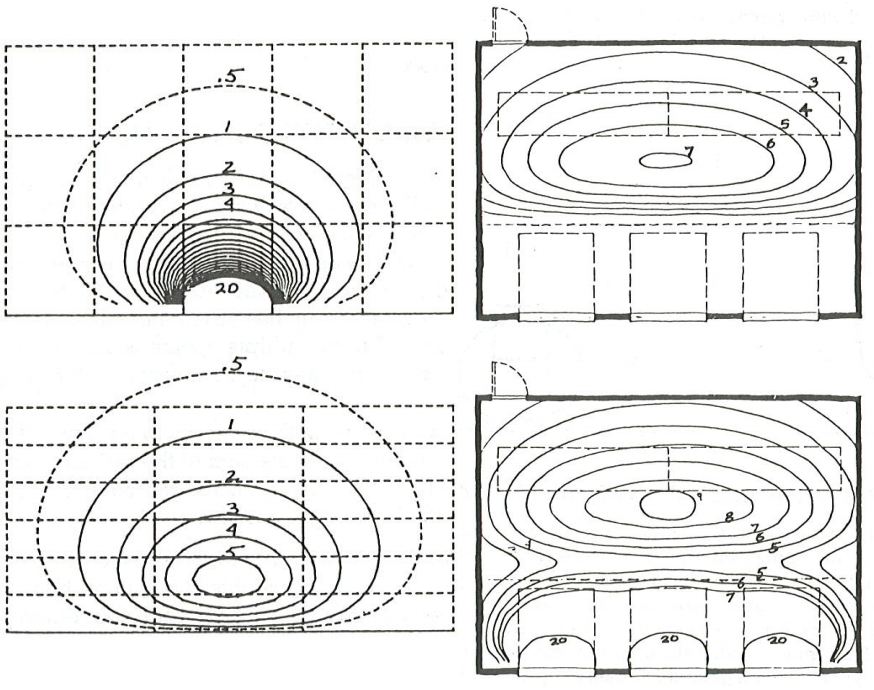
\includegraphics[width=0.5\textwidth]{GDDM_0}
      \caption{This is the overlay used to trace contour lines in the GDDM method. There are many and simple calculations are used to decide which overlay to use.}
      \label{fig:GDDM_0}
    \end{minipage}
    \hfill
    \begin{minipage}[b]{0.4\textwidth}
      \centering
      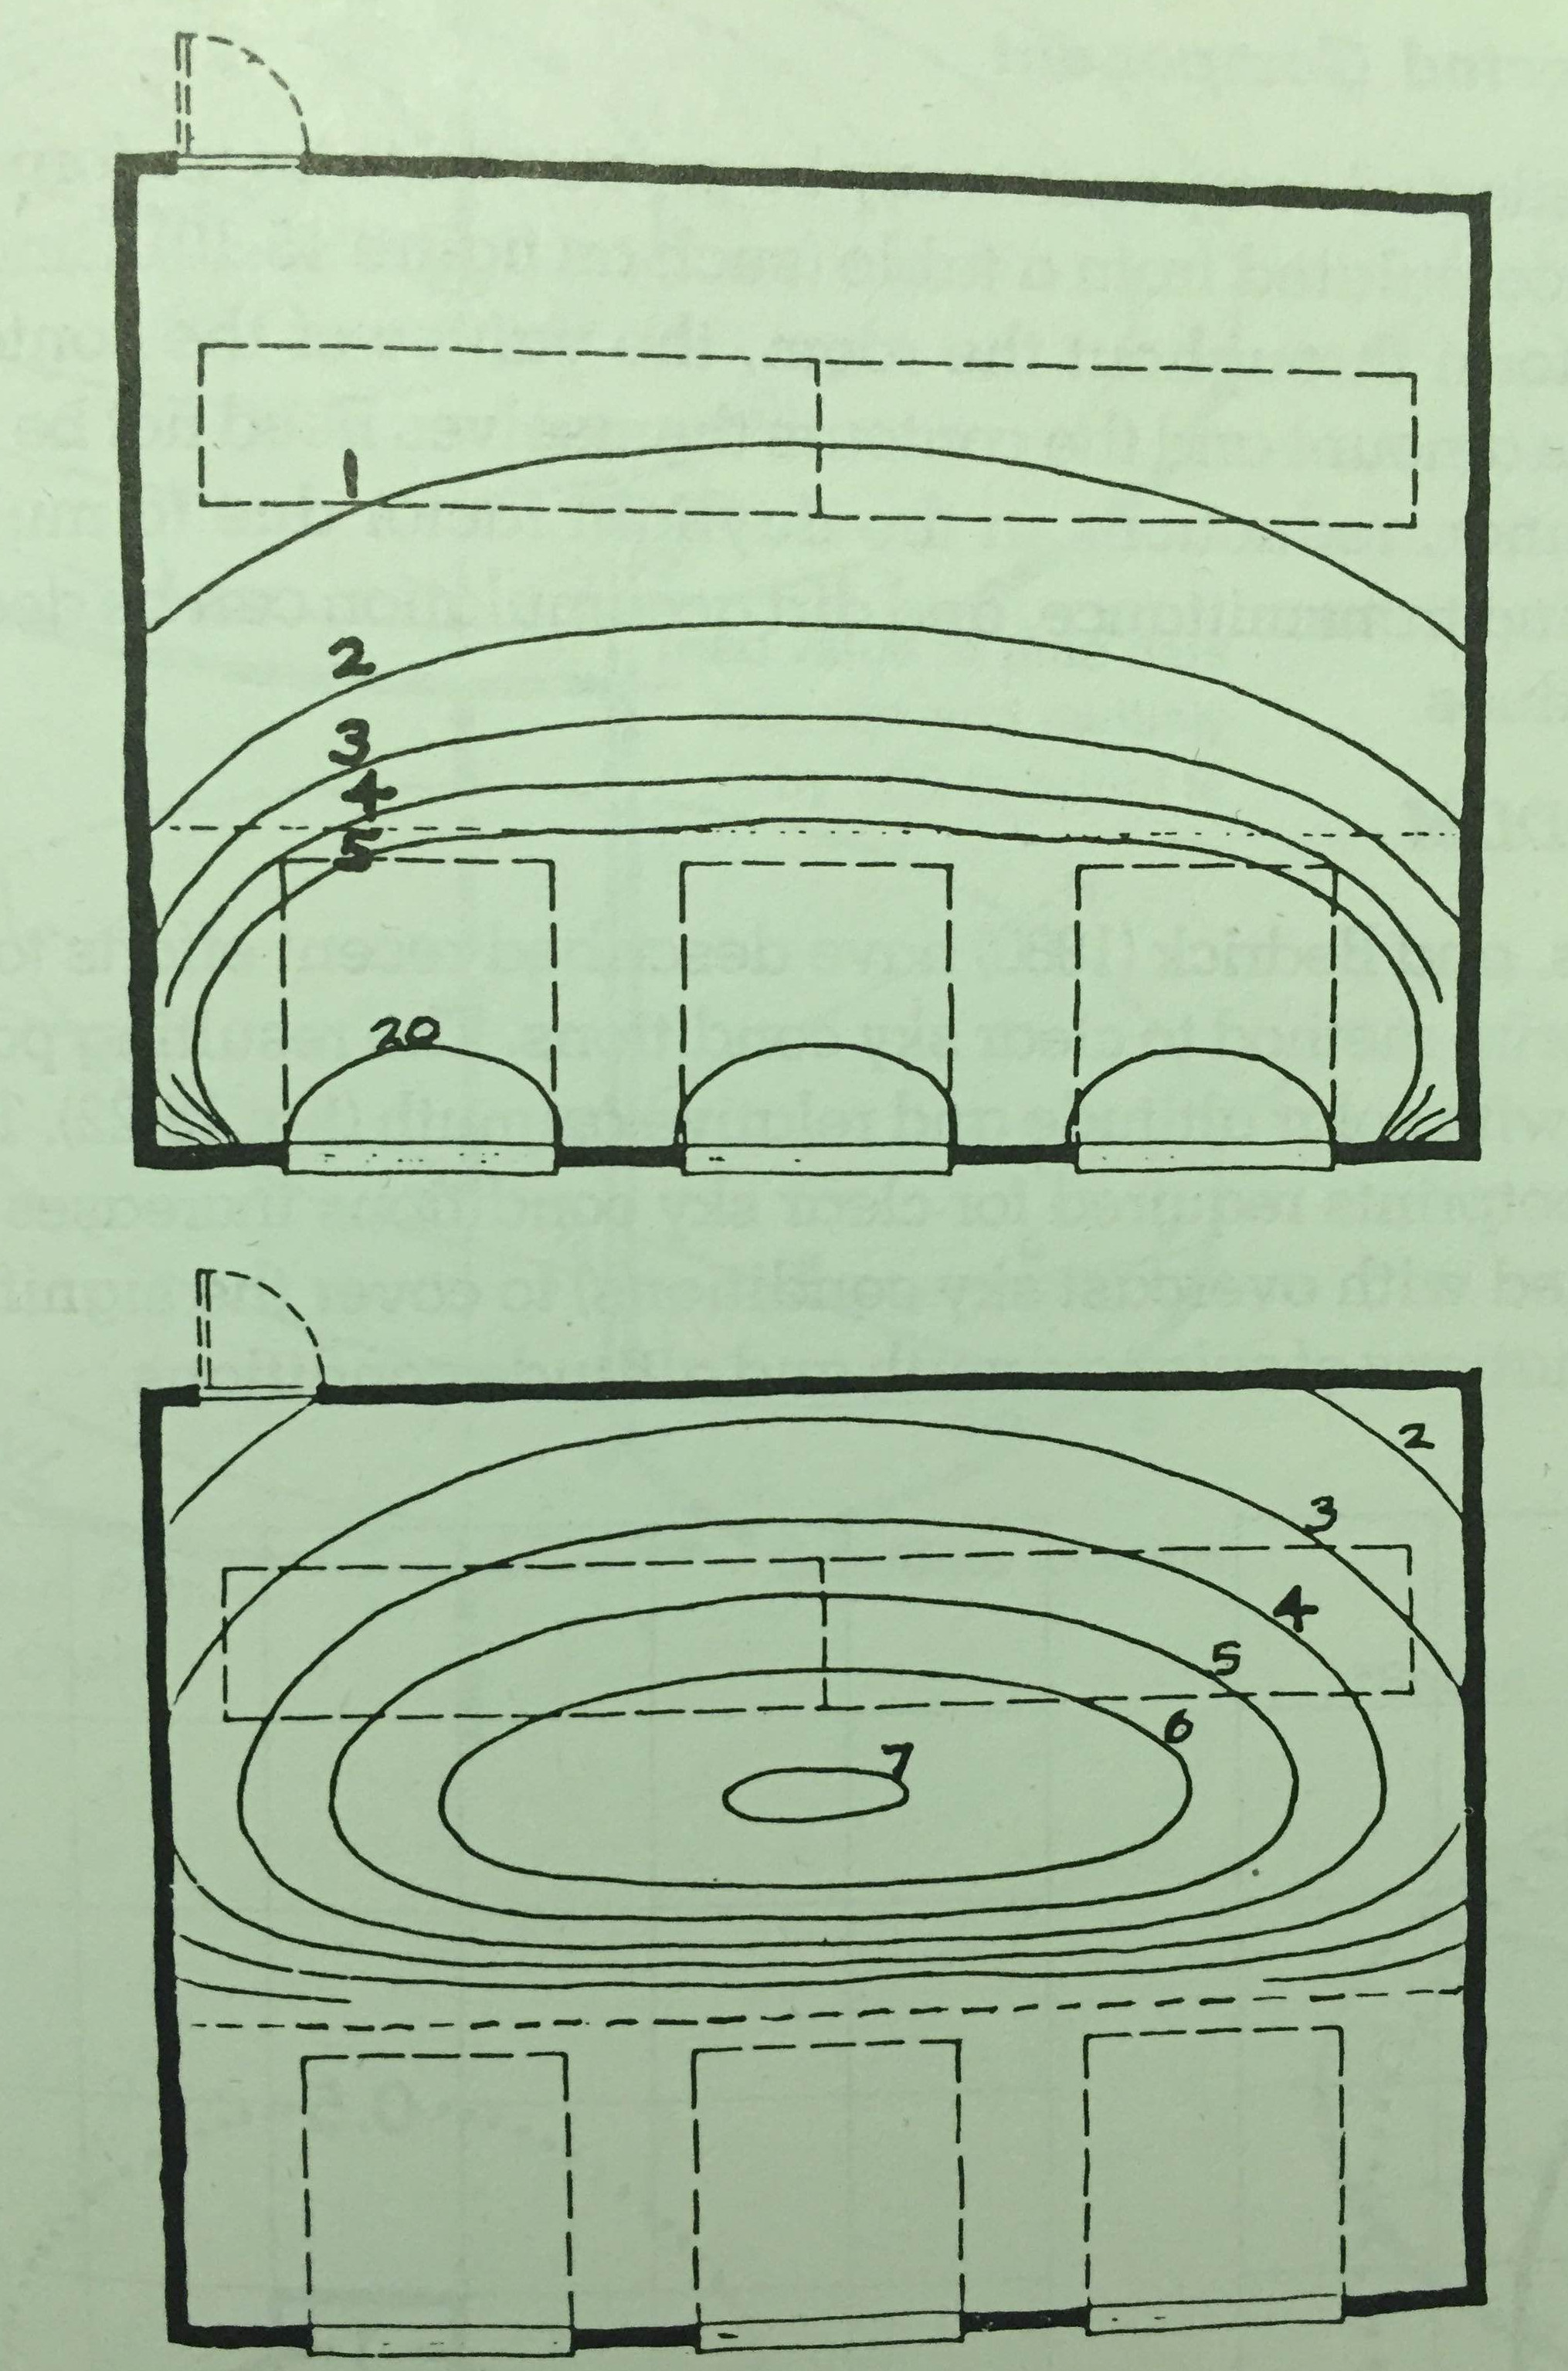
\includegraphics[width=0.5\textwidth]{GDDM_1}
      \caption{This is a finalized sketch with combined overlays show the distributions of daylight in a space.}
      \label{fig:GDDM_1}
    \end{minipage}
  \end{figure}

  % - Mention what floor plans
  % - introduce Graphic daylighting design method as a sketching based analysis tool
  Sketches can also be used for more than just brainstorming general forms and geometries of architectural spaces. 
  Detailed analysis, with the aid of specialized tools, can be done on sketches as well.
  One such method is the Graphic Daylighting Design Method (GDDM)\cite{millet1980graphic,moore}.
  % - graphical method to predict illumination with CIE overcast sky.
  The GDDM method can be used to predict daylight illumination given an overcast sky.
  % - shows luminance and distribution
  The GDDM shows both lighting distribution and intensity through using contour line visualizations.
  % - simple calculations to determine which daylight footprint to use
  To use GDDM, first the architect would draw a floor plan of the room, making note of where windows are located.
  Using a series of specialized transparent overlays the architect can trace contour lines defining both daylighting distribution and intensity such as seen seen in Figure \ref{fig:GDDM_0} and \ref{fig:GDDM_1}.
  These analytical sketches allow architects to evaluate designs and make renovations to improve lighting conditions.
  The GDDM technique and other basic sketch-based brainstorming strategies help architects perform analysis on sketches quickly during the earliest stages of design.

  % - overlay the drawing over your sketch
  % - do this for all light sources in an additive fashion
  % - in the end you get a contour of daylighting
  % - \cite{millet1980graphic}

  % Recap why sketches are widely used still

  % Possible extension, include calculations from:
  % http://tinyurl.com/h4qm5cv

  \subsection{Daylighting After The Early Design Phase}
  % Explain that daylighting effects everything
  Daylight plays a role in every phase of the architectural design process.
  % Explain how in design dev 3D models are made and more analysis is done
  For example, during the design development phase architects will create either scale physical models of a building or create 3D virtual models.
  These models are used for much more detailed analysis compared to analysis during the schematic design phase.
  % Explain how the specifics of the dimming systems are later thought up of
  More information about these detailed daylighting analysis methods is covered in the next chapter.

  % Explain that daylighting covers other phases as well, however we will not cover those because we mostly interested in the early design phase

\section{Chapter Summary}

% Overview 
There are a myriad of motives that draw the attention of architects, building owners, and researchers to daylighting systems.
Research is continuously discovering health benefits of regular exposure to daylight including the promotion of vitamin D synthesis, the suppression of melatonin , and the regulation of the human circadian rhythm.
Additional studies show  that there are economic incentives to implementing daylighting systems.
Some economic incentives come in the form of increases in worker productivity; 
While other economic incentives take the form of energy savings from reducing demand of electrical lighting.
Motivations aside, daylighting systems are difficult to implement due to the dynamic nature of the sun.
The distribution of daylight in an architectural space is dependent on many factors including (but not limited to) the cardinal direction of fenestrations, geometry of architectural spaces, the reflective properties of interior surfaces, and geographic location of a proposed space.
Moreover, daylight varies not only throughout the day, but also throughout the year.
While architects may be tempted to design architectural spaces with many apertures for maximal daylight, architects also have to juggle the risk posed by daylight as well.
Poor choices in daylighting systems can result in discomfort to occupants, as well as lost of capital for building owners.
To help overcome the difficulties of daylighting, architects use a variety of simple rules known as rules-of-thumb during the early stages of design.
For more detailed daylight analysis architects use analytical sketches and techniques to quickly estimate how daylight will be distributed inside of a conceptualized architectural space. 
Current daylighting research is aimed at the creation of daylighting analysis tools that will help architects better handle the challenges posed by daylight.
These daylighting analysis tools are discusses in more detail in the following chapter.
